\addcontentsline{toc}{chapter}{91 - Right triangles with integer coordinates}
\chapter*{91 - Right triangles with integer coordinates}

\index{binary search}
The points $P(x_1, y_1)$ and $Q(x_2, y_2)$ are plotted at integer co-ordinates and are joined to the origin, $O(0,0)$, to form $\Delta OPQ$.

\begin{figure}[H]
    \centering
    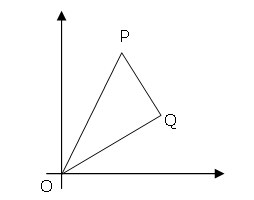
\includegraphics[scale=0.5]{images/pe911.png}
    \caption{}
    \label{fig:pe91a}
\end{figure}

There are exactly fourteen triangles containing a right angle that can be formed when each co-ordinate lies between 0 and 2 inclusive; that is, $0 \leq x1, y1, x2, y2\leq 2$.

\begin{figure}[H]
    \centering
    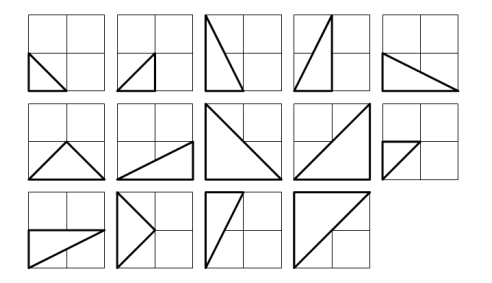
\includegraphics[scale=0.5]{images/pe912.png}
    \caption{}
    \label{fig:pe91b}
\end{figure}

Given that $0 \leq x1, y1, x2, y2 \leq 50$, how many right triangles can be formed?

\section*{Solution}

Since the coordinates are integer numbers in the range of $[0,50]$, a brute force approach will run in $O(n^4)$, with $n=50$ we are talking around six millions of operations, which looks reasonable to run in less than a minute. Now, in order to improve a little bit the running time we will do the following:

\begin{enumerate}
    \item Place the first point $(x_1,y_1)$ in the grid. This will take $O(n^2)$ to go trough the whole grid.
    \item For the other point $(x_2,y_2)$ iterate trough all values in the $y-axis$ and using a binary search obtain the $x-coordinate$, this part will run in $O(n \log n)$. Avoid to count the points where $y_2 = y_1$ and those where $x_2 = x_1$. To identify if we have found a valid coordinate we must check that the following statement is true (cosine law).
    
    $$
    x_1^2 + y_1^2 + (x_2-x_1)^2 + (y_2-y1)^2 - x_2^2 - y_2^2 = 0
    $$
    
    \item After counting the triangles f in step 2, we just need add $3n^2$, which is the number of right triangles with sides parallel to the $x$ and $y$ axis. 
    
\end{enumerate}

The running time of this solution is $O(n^3 \log n)$, which is around $7 \times 10^5$ operations.